\section{Problem 1: DIGITAL HALFTONING}\label{problem-1-digital-halftoning}
\textbf{sample1.png} is given in Figure 1.(a) Please apply several halftoning methods to the given image and provide discussions about the detail of the results.

Original image \nameref{sample1} for question \nameref{problem-1-digital-halftoning}.
\begin{figure}
    \centering
    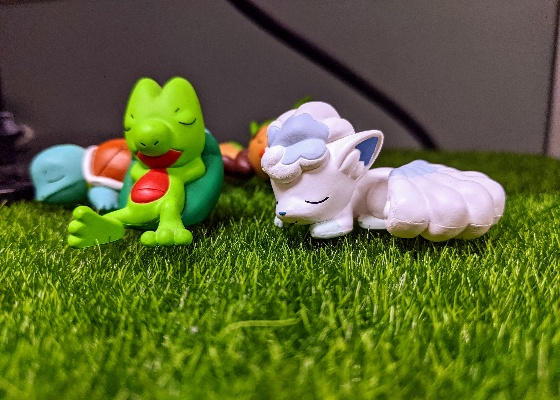
\includegraphics[scale=0.7]{src/sample1.png}
    \caption{\textbf{sample1.jpg}}
    \label{sample1}
\end{figure}

\subsection{(a)}\label{1_a}
Perform dithering using the dither matrix \(I_{2}\) in Figure 1.(b) and output the result as \textbf{result1.png}

\paragraph{Motivation}
Render the illusion of a continuous-tone image based on half-tone (black and white only) display. \textbf{Dithering} methods could create an image with the same size of the original image. So we could start form dither matrix with \(I_{2}\).

\paragraph{Approach}
Follow the steps in \textbf{Lec 6 page 11}.
\begin{enumerate}
    \item Add noise \(N(j, k)\) to get \(H(j, k)\). I only implement \textbf{white noise} with \texttt{np.random.normal(0, 0.05}. Other noise type generator could reference \href{https://stackoverflow.com/questions/67085963/generate-colors-of-noise-in-python}{Generate colors of noise in Python}.
    \item Use dither matrix \(I_{2}\) to generate a threshold matrix \(T^{(2)}_{2}(j, k)\).
    \item Repeat threshold matrix to \(T^{(2)}_{256}(j, k)\) with the same size with original image.
    \item Dither by threshold matrix \(T^{(2)}_{256}\) to get binary output \(G(j, k)\).
\end{enumerate}

\paragraph{Performance of results}
In the end, given dither matrix 
\(
I_{2} = 
\begin{bmatrix}
    1 & 2\\
    0 & 3
\end{bmatrix}
\), and white noise \(N(j, k) = \mathcal{N}(0, 0.05)\).

Result of problem 1(a): \nameref{result1}.
\begin{figure}
    \centering
    \includegraphics[scale=0.7]{src/result1.png}
    \caption{\textbf{result1.jpg} Dithering with \(I_{2}\)}
    \label{result1}
\end{figure}

\paragraph{Discussion}

\subsection{(b)}\label{1_b}
Expand the dither matrix \(I_{2}\) to \(I_{256}\) \((256 \times 256)\) and use it to perform dithering. Output the result as \textbf{result2.png}. Compare \textbf{result1.png} and \textbf{result2.png} along with some discussions.

\paragraph{Motivation}
Apart from `Repeat threshold matrix' in step 3. We could create \(N \times N\) dither matrix based on general form from \(I_{2} \rightarrow I_{4} \rightarrow \dots\).

\paragraph{Approach}
Follow the steps in \textbf{Lec 6 page 16}.
\begin{enumerate}
    \item Design one-step expand with \texttt{expandonce\_dither\_mat}. Use \texttt{np.block} to generate block of sub-array. \\
	\(
	I_{2n}(i, j) = 
	\begin{bmatrix}
	    4 I_{n}(i, j) + 1 & 4 I_{n}(i, j) + 2\\
	    4 I_{n}(i, j) + 3 & 4 I_{n}(i, j) + 0
	\end{bmatrix}
	\)
    \item Repeatedly \(I_{2}\) to \(I_{256}\) as the same size as \nameref{sample1}.
\end{enumerate}

\paragraph{Performance of results}
In the end, I choose the same settings as \ref{1_a} to get \(I_{256}\) as well as \(T^{(256)}_{256}\).

Result of problem 1(b): \nameref{result2}.
\begin{figure}
    \centering
    \includegraphics[scale=0.7]{src/result2.png}
    \caption{\textbf{result2.jpg} Dithering with \(I_{256}\)}
    \label{result2}
\end{figure}

\paragraph{Discussion}
Compare \textbf{result1.png} and \textbf{result2.png}.

\nameref{result1} generate half-tone with more \(\times\) black patterns.

\nameref{result2} sketch fine and smooth on the \textit{face of the cat}. But it shows more scatter black patterns around \textit{cheek (臉頰) and mouth}.

\subsection{(c)}\label{1_c}
Perform error diffusion with two different filter masks. Output the results as \textbf{result3.png}, and \textbf{result4.png}, respectively. Discuss these two masks based on the results. \\
You can find some masks \textbf{here} (from lecture slide 06. p23)

\paragraph{Motivation}
The \textbf{error diffusion} is a practical algorithm to implement \textbf{blue noise dithering}.

\paragraph{Approach}
Follow the steps in \textbf{Lec 6 page 23---24}.
\begin{enumerate}
    \item Generate \textbf{filter mask}. I implement \textbf{Floyd Steinberg} and \textbf{Jarvis} filter mask.
    \item Error diffusion with serpentine scanning. As start from \texttt{i = 0}, I reverse order when \texttt{i \% 2 == 1} is odd.
\end{enumerate}

\paragraph{Performance of results}
In the end, I choose the settings with threshold \(t = 0.5\).

For \textbf{Floyd Steinberg},
result of problem 1(c): \nameref{result3}.
\begin{figure}
    \centering
    \includegraphics[scale=0.7]{src/result3.png}
    \caption{\textbf{result3.jpg} Error diffusion with mask Floyd Steinberg}
    \label{result3}
\end{figure}

For \textbf{Jarvis},
result of problem 1(c): \nameref{result4}.
\begin{figure}
    \centering
    \includegraphics[scale=0.7]{src/result4.png}
    \caption{\textbf{result4.jpg} Error diffusion with mask Jarvis}
    \label{result4}
\end{figure}

\paragraph{Discussion}
Discuss \textbf{Floyd Steinberg} \& \textbf{Jarvis} based on the results.

\textbf{Floyd Steinberg}: It seems \(\times\) black patterns on the \textit{neck}.

\textbf{Jarvis}: It seems more \textbf{twist} black patterns around the face. But I do not like its \textit{left eye} with some \textbf{cluster} of whit patterns.

Both of \textbf{Floyd Steinberg} \& \textbf{Jarvis} sketch \textit{beards} more clear. And I feel \textbf{Floyd Steinberg} is more clear in its \textit{six-line beards}.

I find out that baoundary of my image has some white line patterns. I consider that it occurs as I don't conduct padding of this image.

Other masks.
I try other maske 
\(
\tilde{D} = \frac{1}{2}
\begin{bmatrix}
    - & \bullet & 1\\
    - & 1  & 0
\end{bmatrix}
\) 
result of problem 1(c): \nameref{result1c_diag}.
\begin{figure}
    \centering
    \includegraphics[scale=0.7]{src/tmp/result1c_diag.png}
    \caption{\textbf{result1c\_diag} Error diffusion with mask \(\tilde{D}\)}
    \label{result1c_diag}
\end{figure}
This simple mask makes less contrast than \textbf{Jarvis} but seems better on its eyes for me.

%\alert{Mistake} with create new empty to assign the error difussion value.

\subsection{(d)}\label{1_d}
Try to transfer \textbf{result1.png} to a dotted halftone/manga style binary image such as \textbf{sample1\_dotted.png} in Figure 1.(c). Describe the steps in detail and show the result. \\
You may need to utilize a function like \textbf{cv2.circle} to draw a circle.

\paragraph{Motivation}
It is interesting approach of \textbf{dotted halftone} / \textbf{manga style}.

\paragraph{Approach}
Rather than use \texttt{cv2.circle}, I use \texttt{PIL.ImageDraw} object with its \texttt{ellipse()} method.
\begin{enumerate}
    \item Create new canvas as the same size of original binary image.
    \item Design the kernel matrix \(K_{3 \times 3}\) with siez \(3\).
    \item Calculate \textbf{mean} of sub-array \(\bar{H}\)  by convolution of \(K_{3 \times 3}\) then add white noise \(N_{3 \times 3} \sim \mathcal{N}(0, 0.05)\) .
    \item Design \textbf{different radius} circle patterns based on the rules.
	\[
	    r = 
	    \begin{cases}
		0 ,& \text{if } \bar{H} \leq 0.2\\
		1 ,& \text{if } 0.2 < \bar{H} \leq 0.4\\
		2 ,& \text{if } 0.4 < \bar{H} \leq 0.6\\
		3 ,& \text{if } 0.6 < \bar{H} \leq 0.8\\
	        4 ,& \text{if } 0.8 < \bar{H} \leq 1
	    \end{cases}
	\]
	Note when radius \(r=4\), it means \textbf{square pattern} rather than \textbf{circle pattern} of sub-array.
    \item Draw with \texttt{draw.ellipse((x-left, y-top), (x-right, y-bottom), radius, fill="white" )}  
\end{enumerate}

\paragraph{Performance of results}
In the end, based on \nameref{result1}.

Result of problem 1(d): \nameref{sample1dotted.png}.
\begin{figure}
    \centering
    \includegraphics[scale=0.7]{src/sample1_dotted.png}
    \caption{\textbf{sample1\_dotted.png} Dotted halftone style transfer}
    \label{sample1dotted.png}
\end{figure}

\paragraph{Discussion}
Interesting style transfer methods. We could apply it on different dithering results, binary image.
And design new patterns in the future.

